\subsubsection{Detalles de la actividad}
Siguiendo las buenas practicas de Next.js dice que deberias realizar un componente que debuelve al componente padre siguiente este paradigma creamos la pagina principal con sus componentes de navegador, encabezado, carrusel y sus modelos para cada sub unidad.
creamos esos componentes y lo colocamos con datos ficticios por el momento hasta que salga los enpoints de la parte de backend y poder conectarlo con el fronted.
Enlace del fronted en GitHub \href{https://github.com/brahyanarch/frontend-next-dpsec.git}{https://github.com/brahyanarch/frontend-next-dpsec.git}
Para comprobar en la parte de logs la parte de pagina principal.


\begin{figure}[!htb] 
    \centering 
    \caption{Configuracion de un nuevo proyecto en Next.js} 
    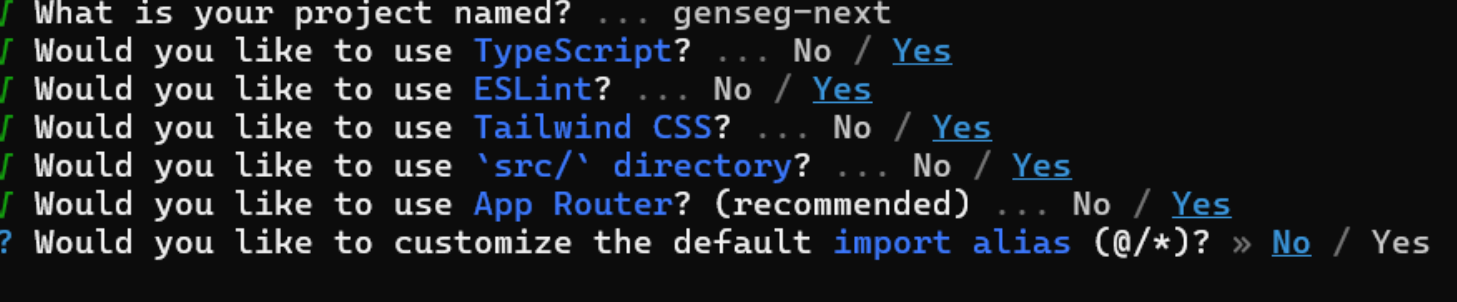
\includegraphics[width=0.8\textwidth]{assets/imagenes/config_next.png}
    \label{fig:config_next} 
\end{figure} 
\FloatBarrier

\begin{figure}[!htb] 
    \centering 
    \caption{Todo okey para trabajar en Next.js} 
    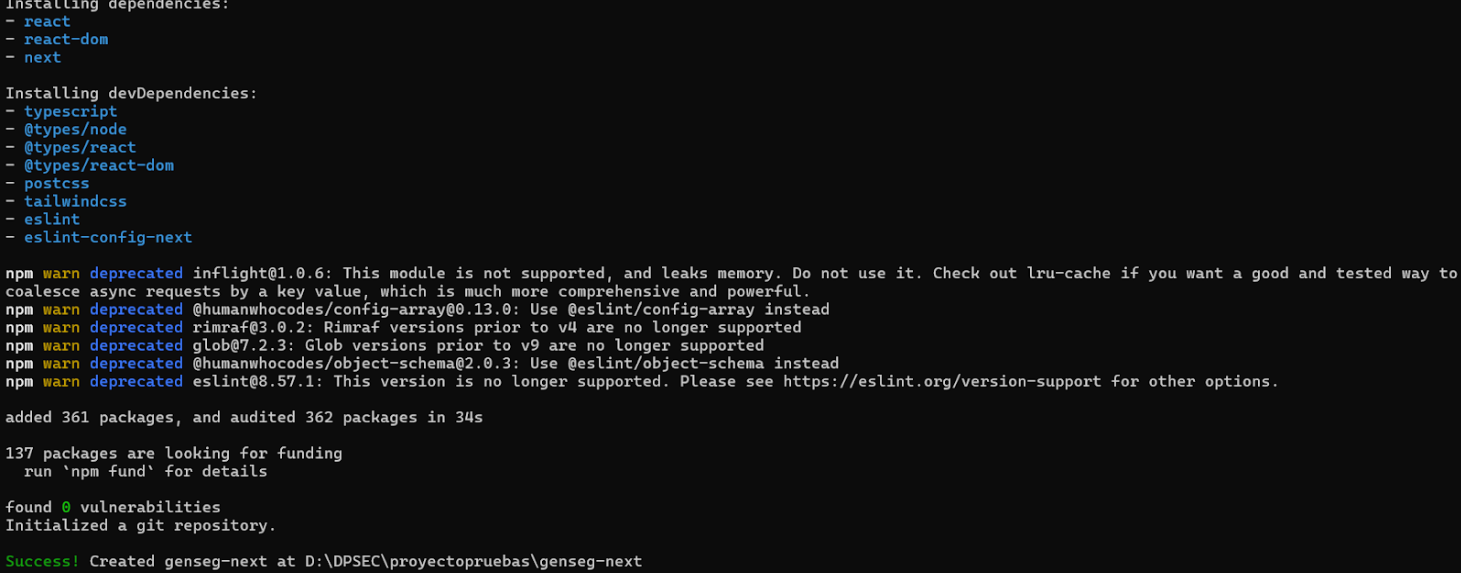
\includegraphics[width=0.8\textwidth]{assets/imagenes/next_listo.png}
    \label{fig:listo_next} 
\end{figure} 
\FloatBarrier


\begin{lstlisting}[language=Python, caption=Inicializando el proyecto en Next.js, label={lst:next}]
    > npm run dev
    
    > project-genseg@0.1.0 dev
    > next dev
    
    Port 3000 is in use, trying 3001 instead.
    Next.js 14.2.9
    - Local:        http://localhost:3001
    - Environments: .env
    
    Starting...
    Ready in 4.4s
\end{lstlisting}


\begin{figure}[!htb] 
    \centering 
    \caption{Ejecutando en el navegador} 
    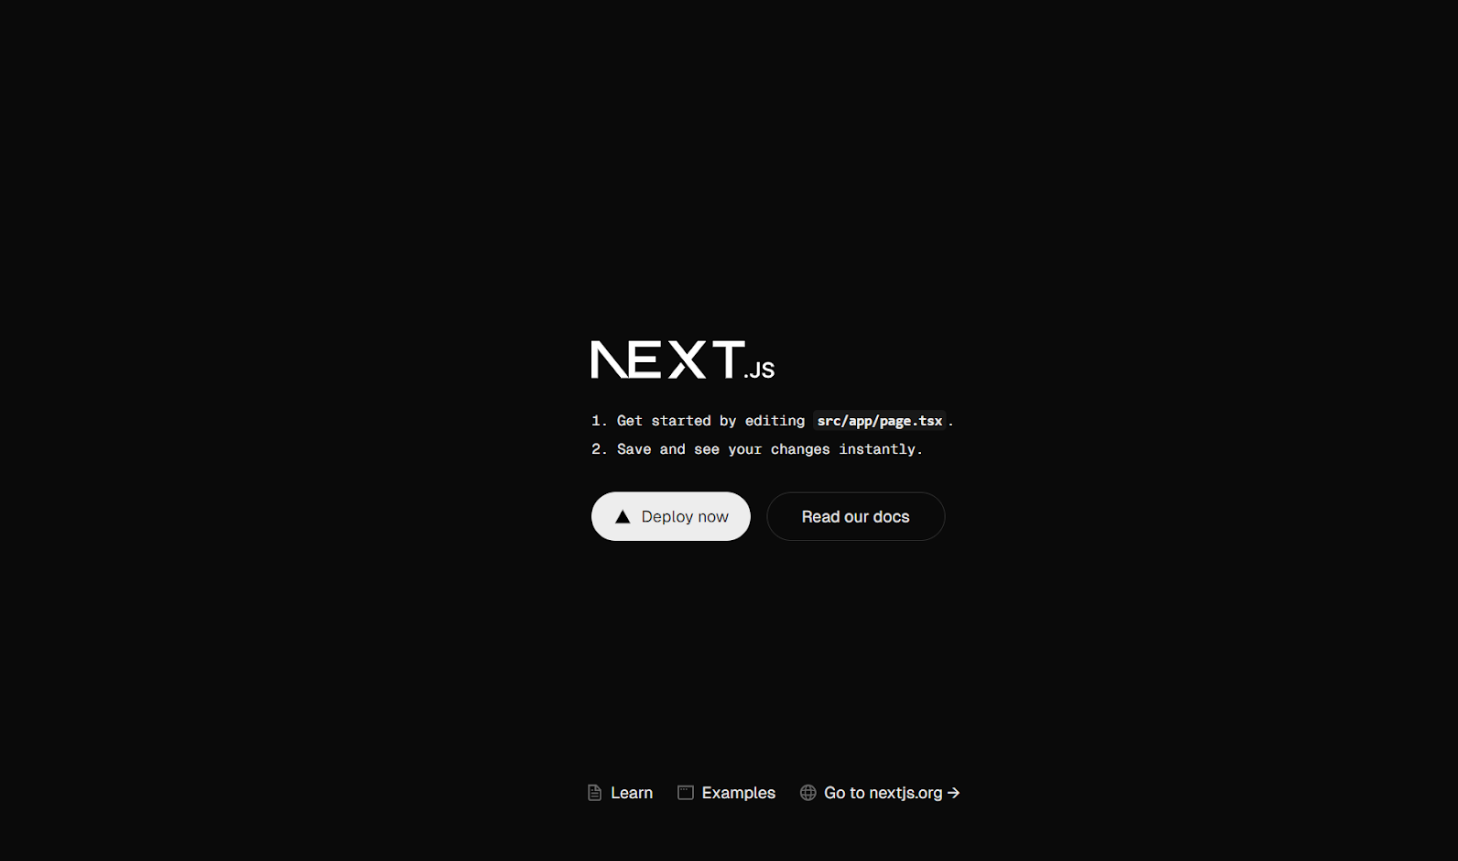
\includegraphics[width=0.8\textwidth]{assets/imagenes/init_next.png}
    \label{fig:init_next} 
\end{figure} 
\FloatBarrier

\begin{figure}[!htb] 
    \centering 
    \caption{Codigo en Visual Studio Code} 
    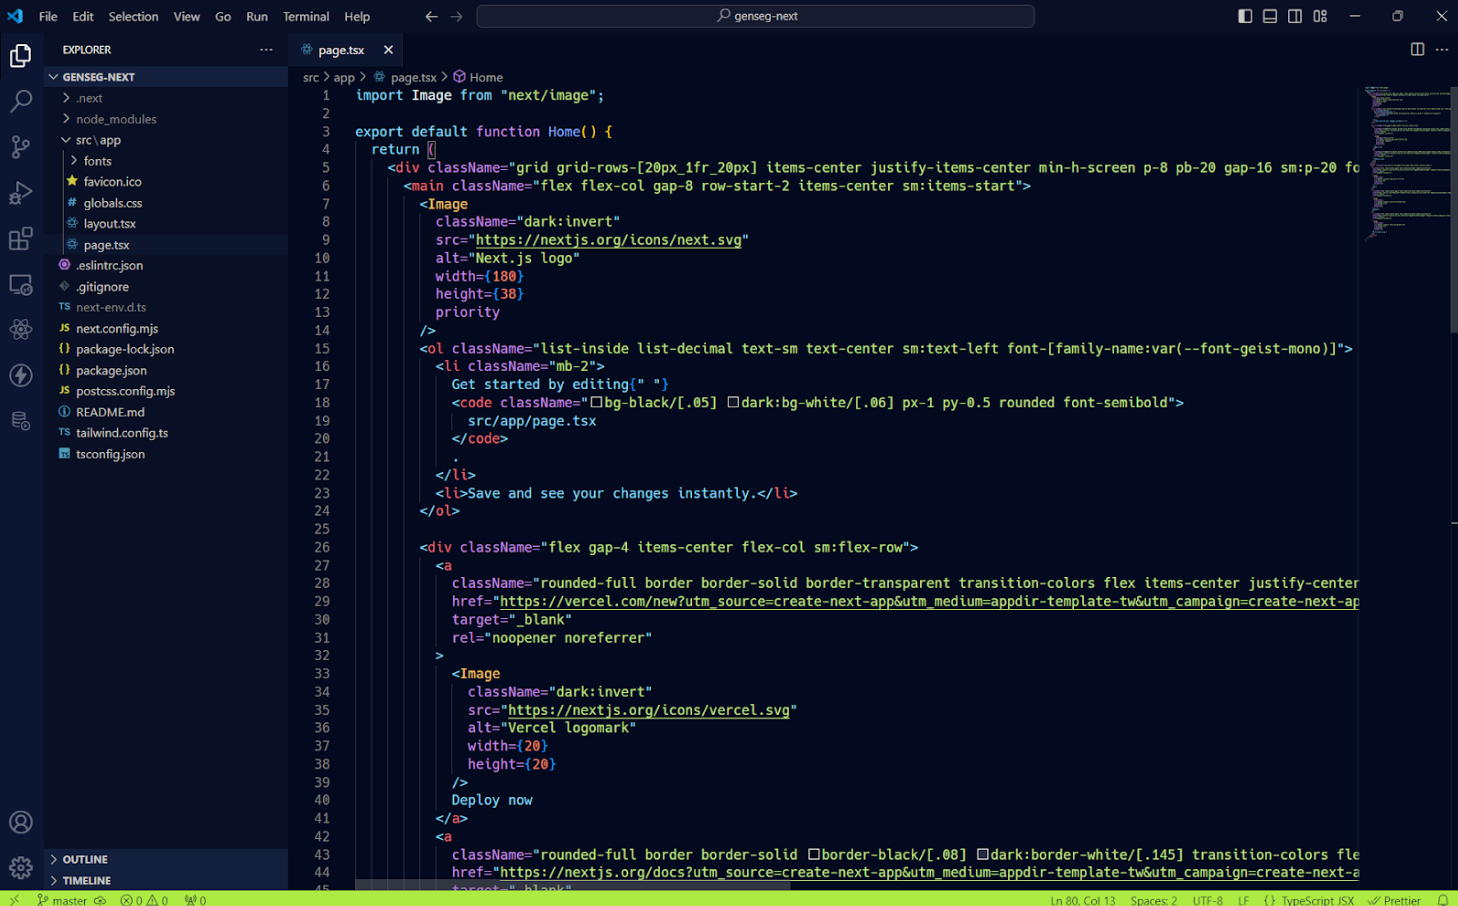
\includegraphics[width=0.8\textwidth]{assets/imagenes/vista_codigo.png}
    \label{fig:codigo} 
\end{figure} 
\FloatBarrier

\begin{figure}[!htb] 
    \centering 
    \caption{Pagina principal codificado} 
    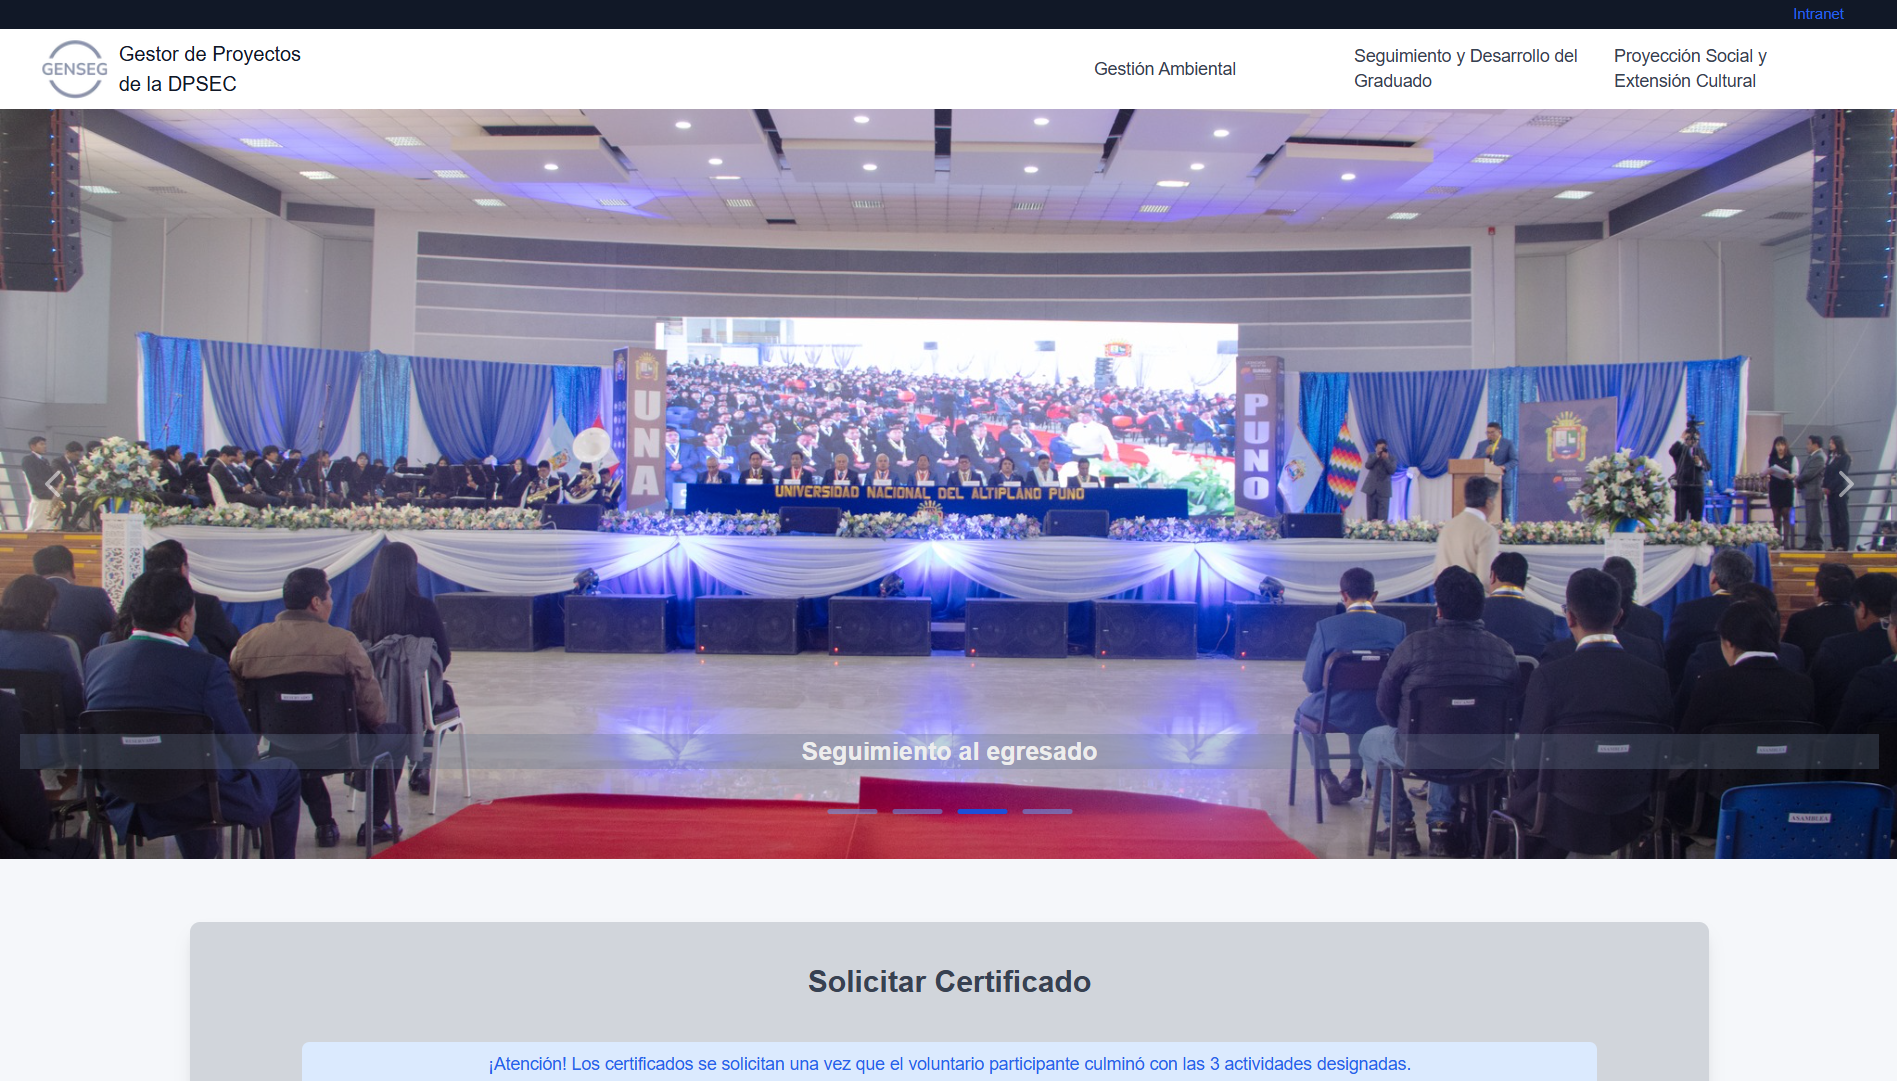
\includegraphics[width=0.8\textwidth]{assets/imagenes/paginaprincipalCodigo.png}
    \label{fig:pagina_codificado} 
\end{figure} 
\FloatBarrier


\begin{figure}[!htb] 
    \centering 
    \caption{Pagina login} 
    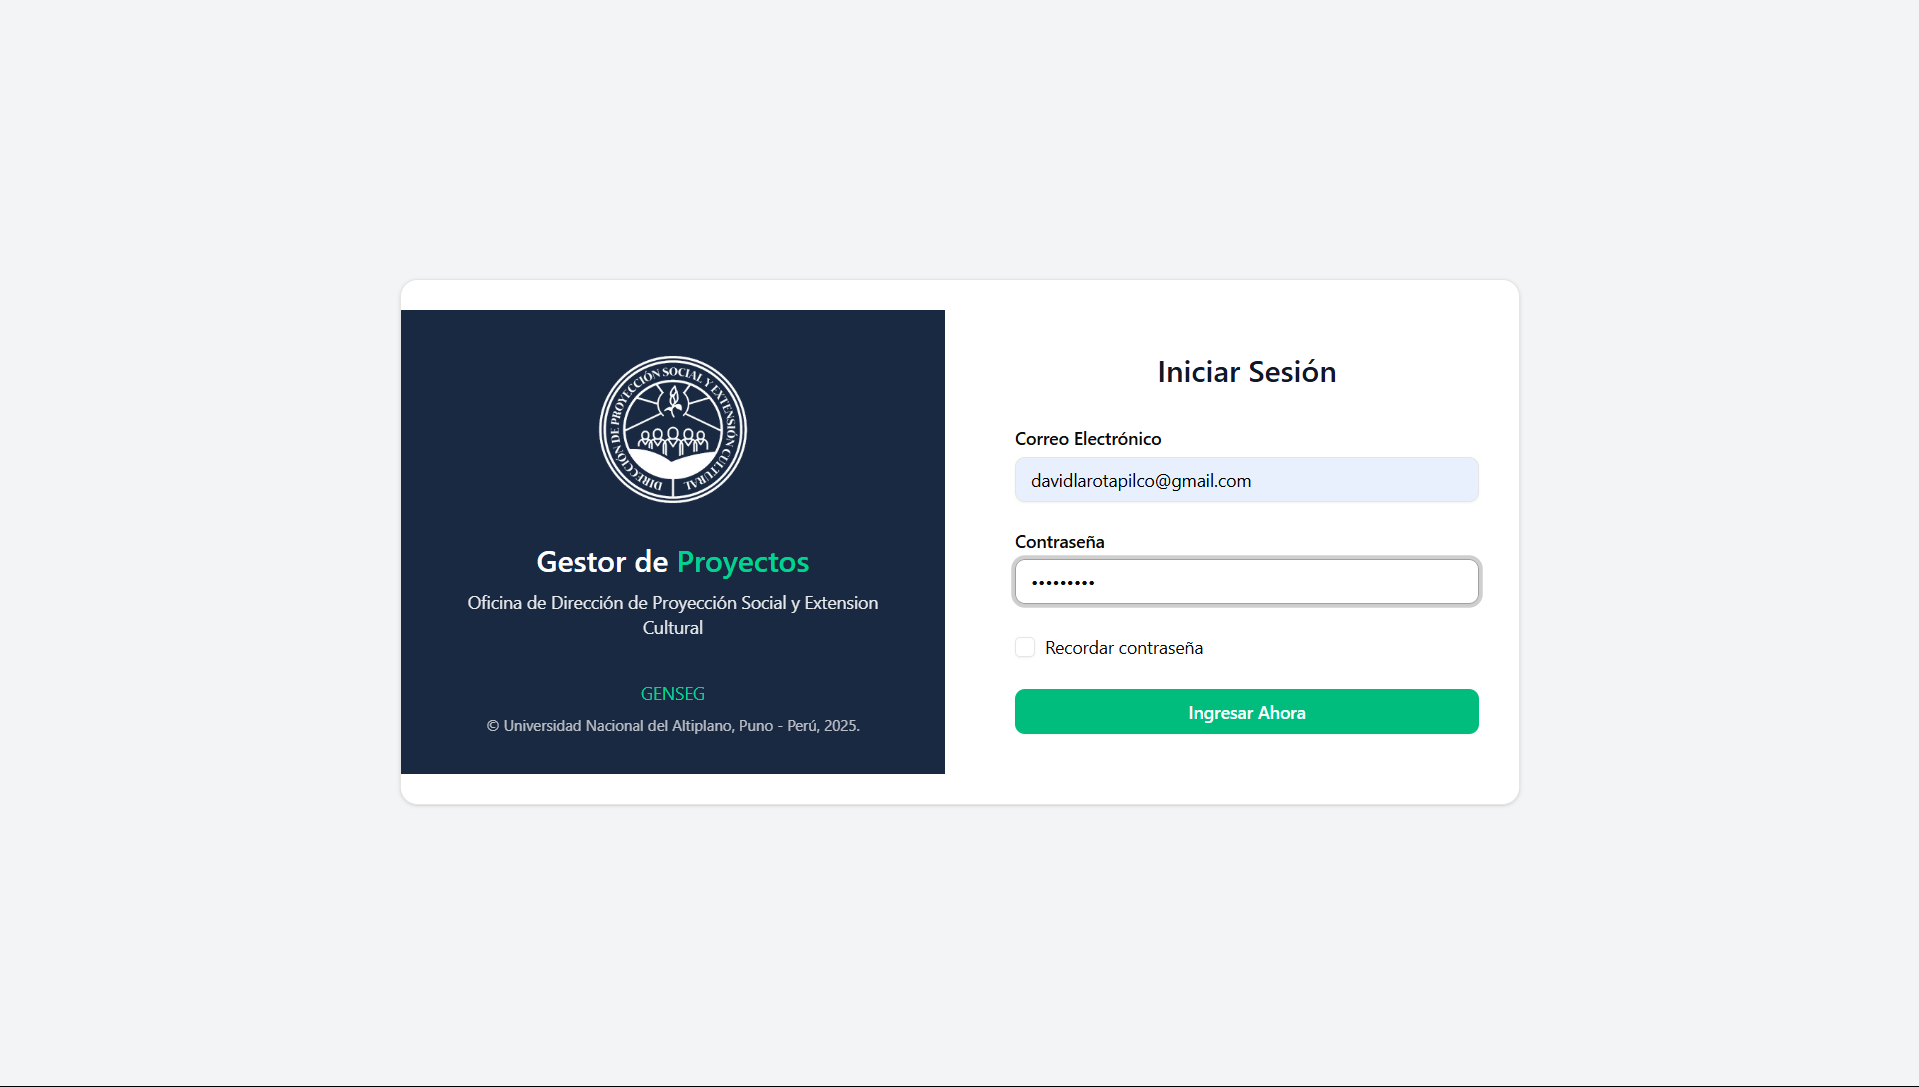
\includegraphics[width=0.8\textwidth]{assets/imagenes/login.png}
    \label{fig:login} 
\end{figure} 
\FloatBarrier

\begin{figure}[!htb] 
    \centering 
    \caption{Pagina escoger rol} 
    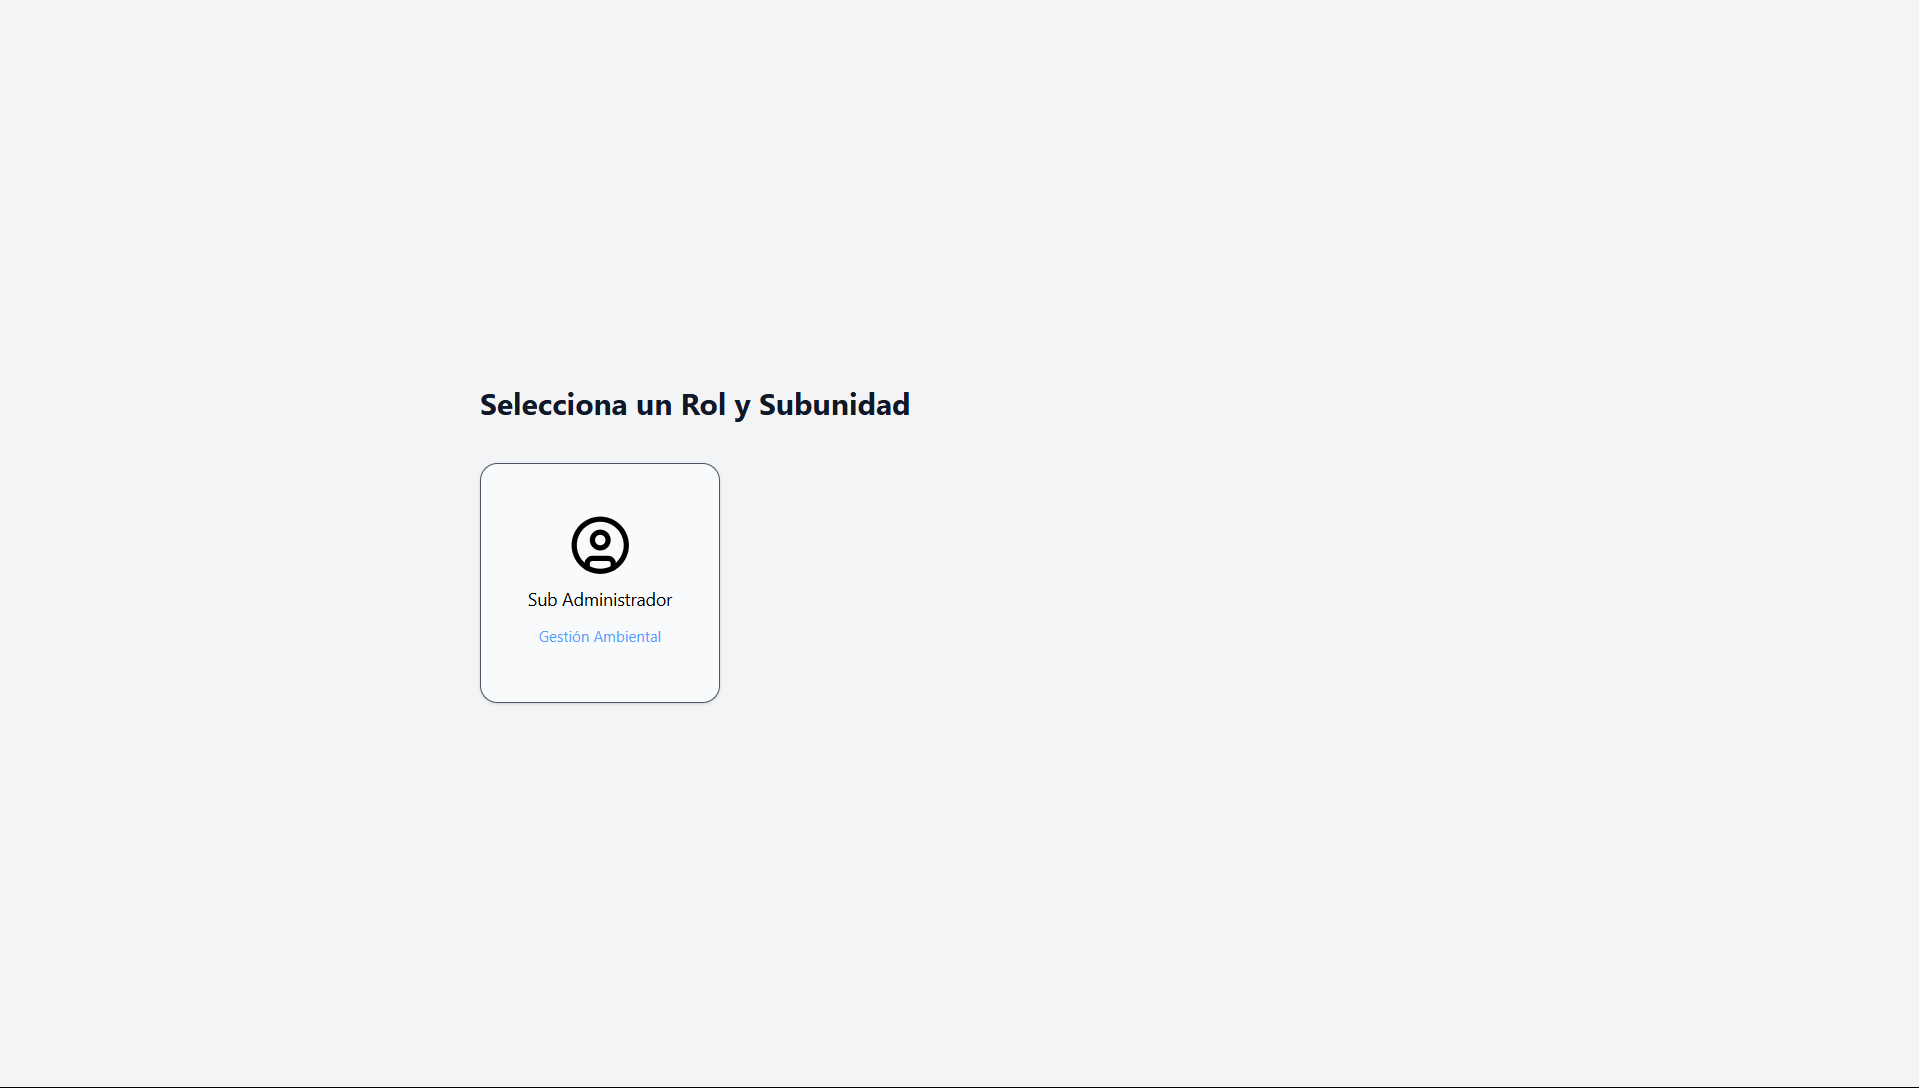
\includegraphics[width=0.8\textwidth]{assets/imagenes/rol.png}
    \label{fig:rol} 
\end{figure} 
\FloatBarrier
\begin{figure}[!htb] 
    \centering 
    \caption{Pagina para gestionar formularios} 
    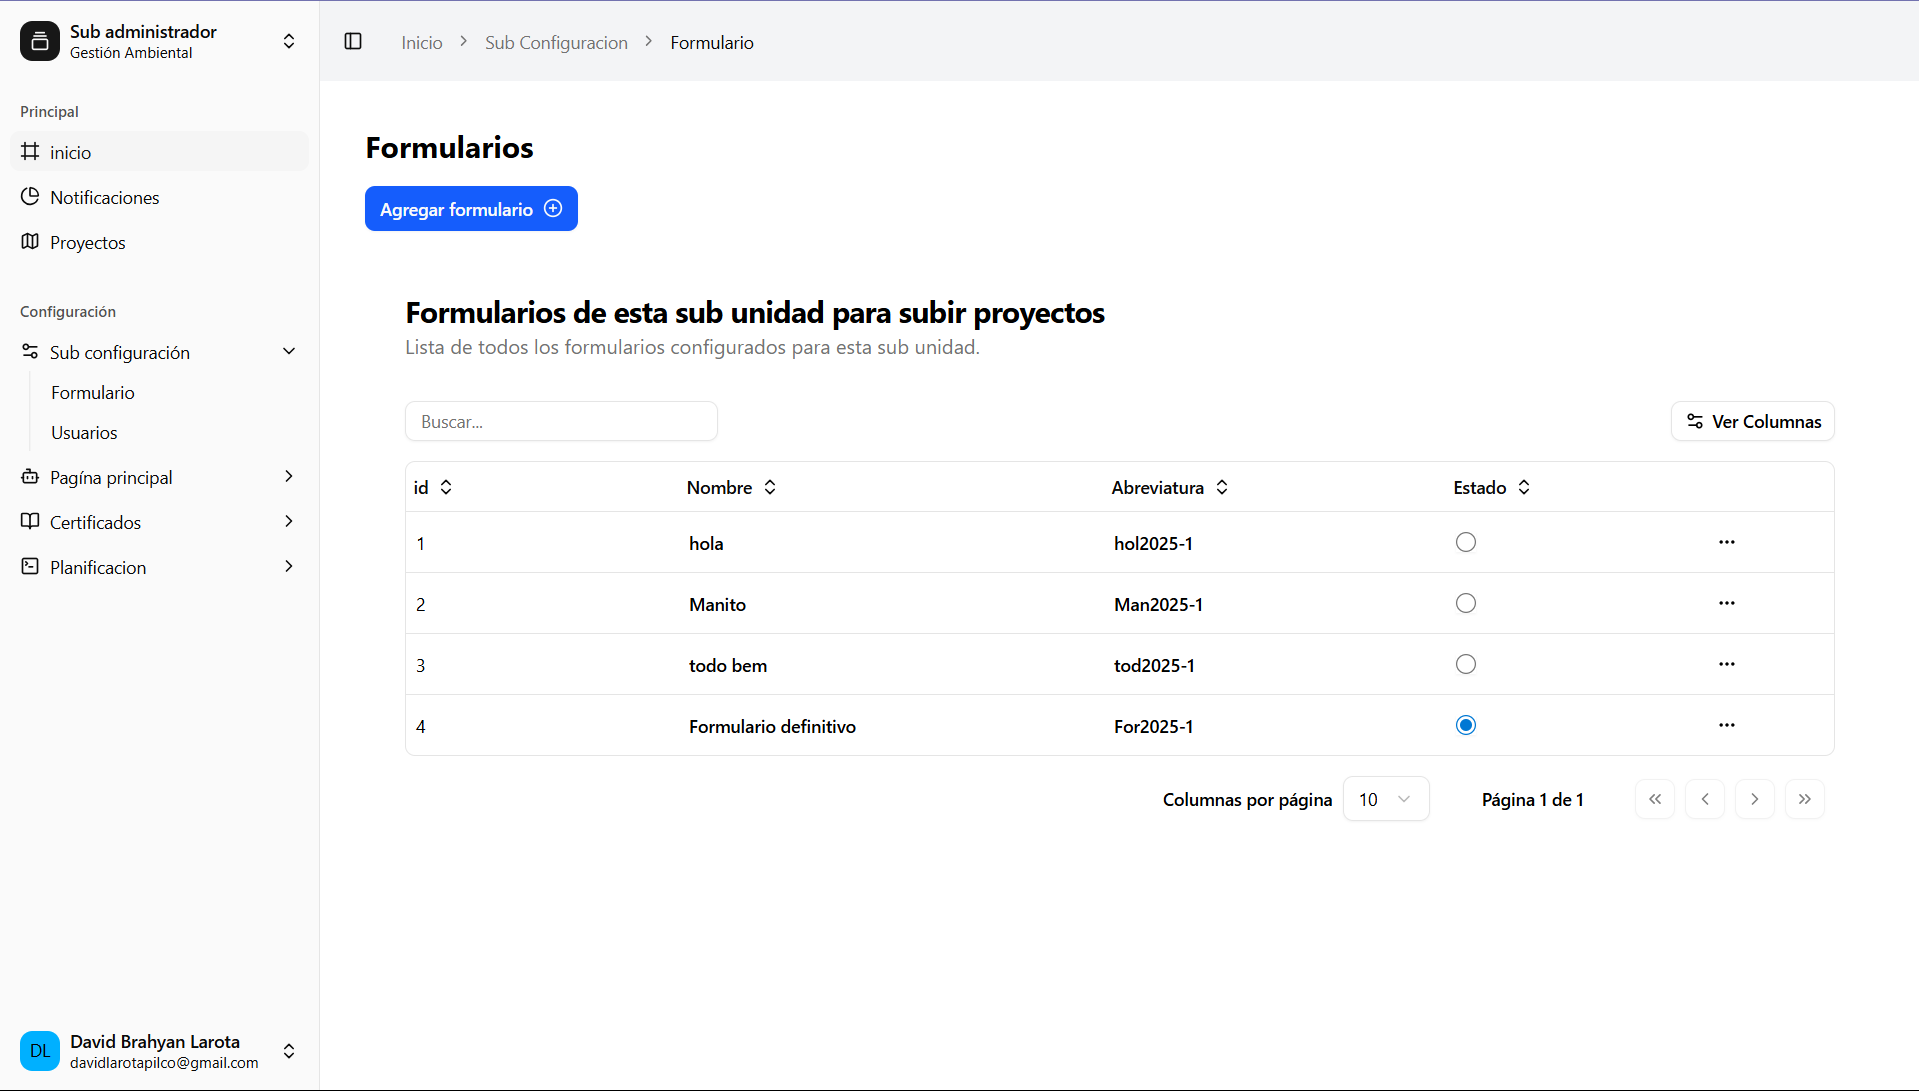
\includegraphics[width=0.8\textwidth]{assets/imagenes/formularios.png}
    \label{fig:formularios} 
\end{figure} 
\FloatBarrier
\begin{figure}[!htb] 
    \centering 
    \caption{Pagina para crear preguntas} 
    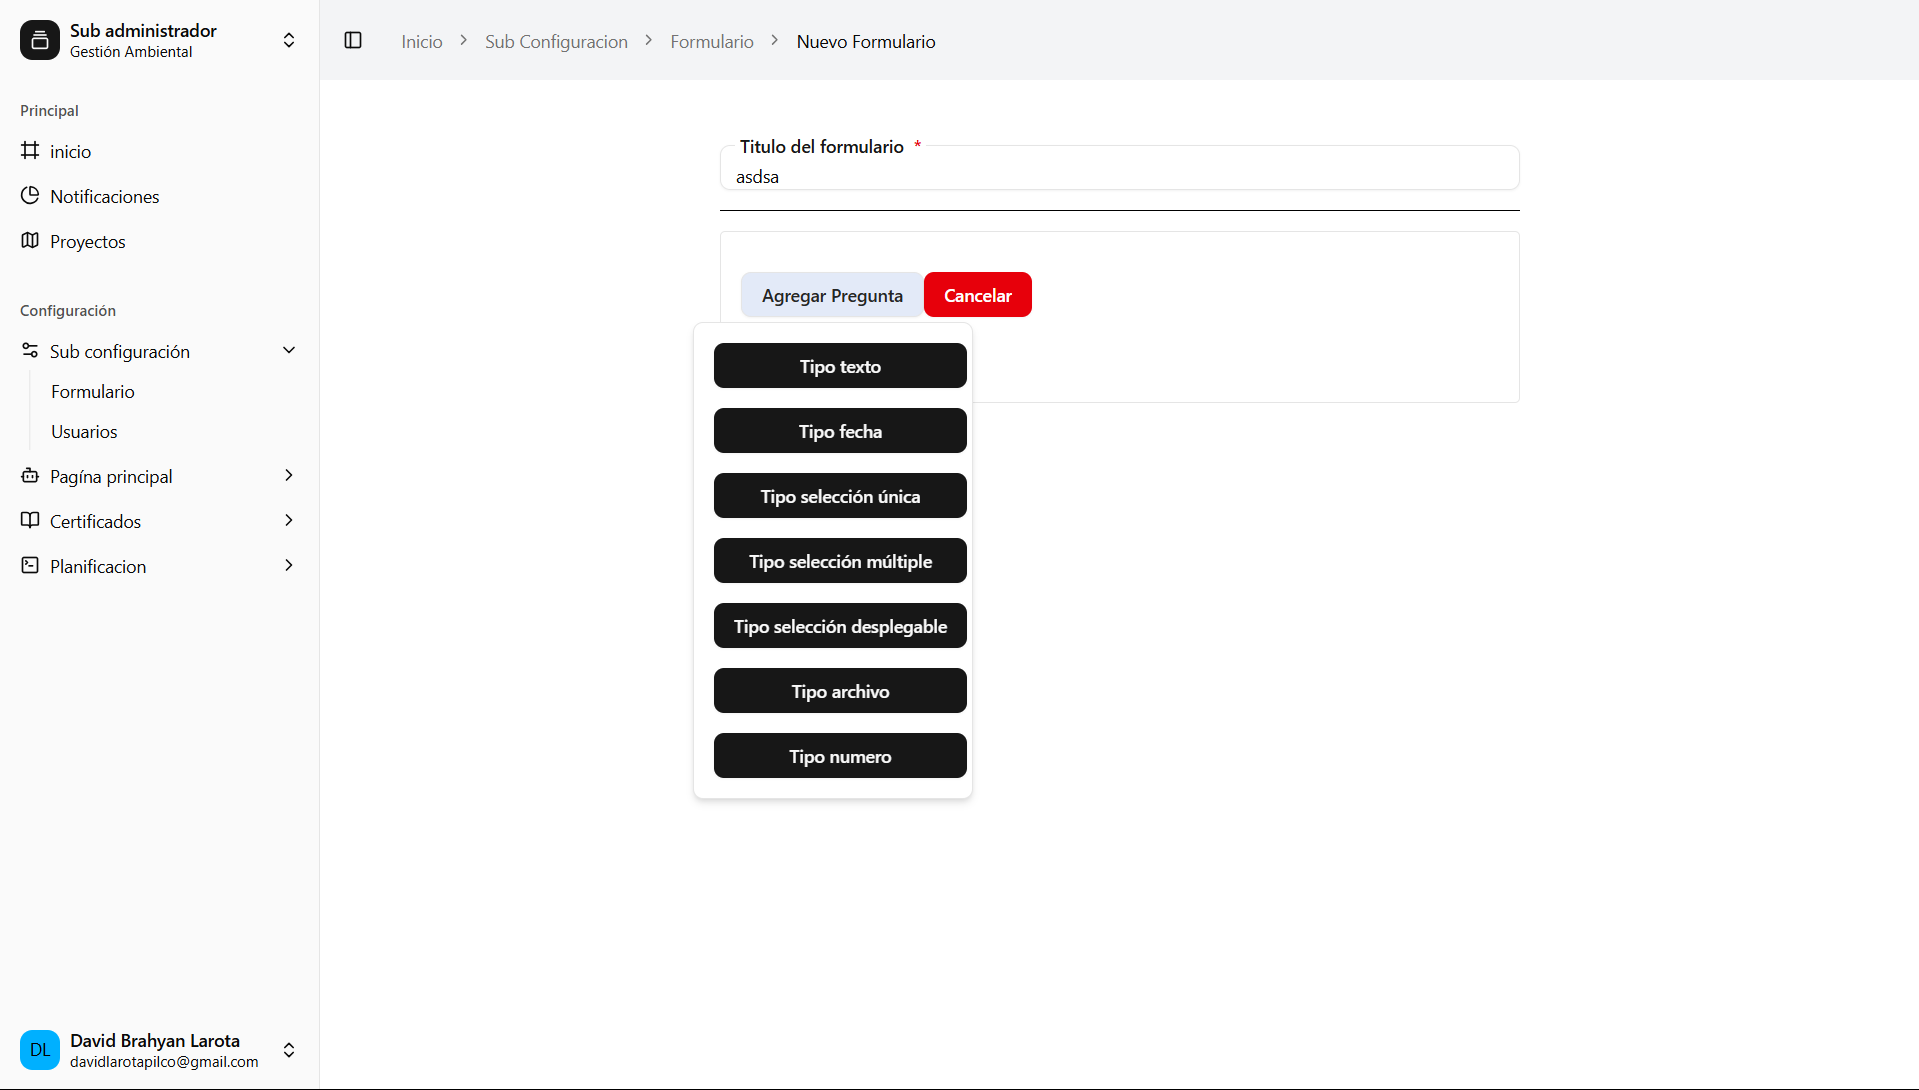
\includegraphics[width=0.8\textwidth]{assets/imagenes/preguntas.png}
    \label{fig:preguntas} 
\end{figure} 
\FloatBarrier
\begin{figure}[!htb] 
    \centering 
    \caption{Pagina para gestionar usuarios} 
    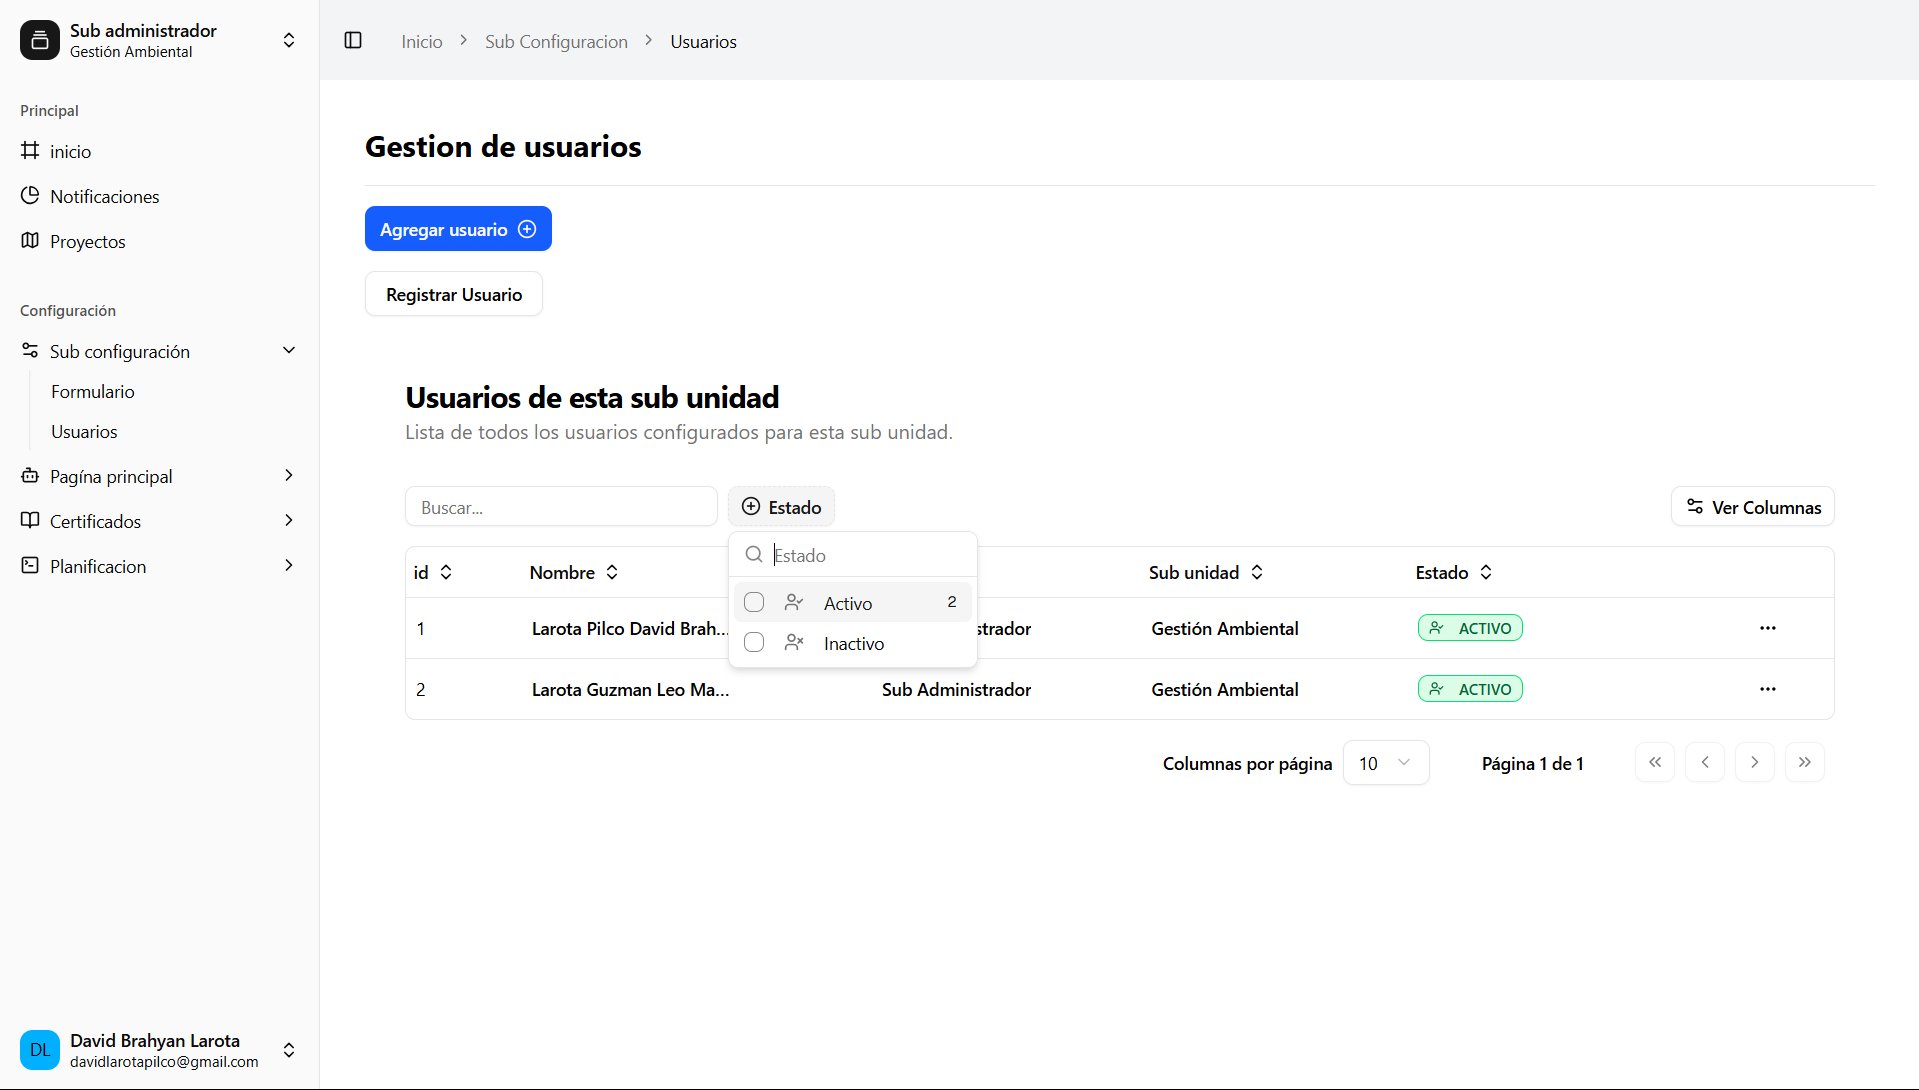
\includegraphics[width=0.8\textwidth]{assets/imagenes/usuarios.png}
    \label{fig:usuarios} 
\end{figure} 
\FloatBarrier
\begin{figure}[!htb] 
    \centering 
    \caption{Pagina para proyectos} 
    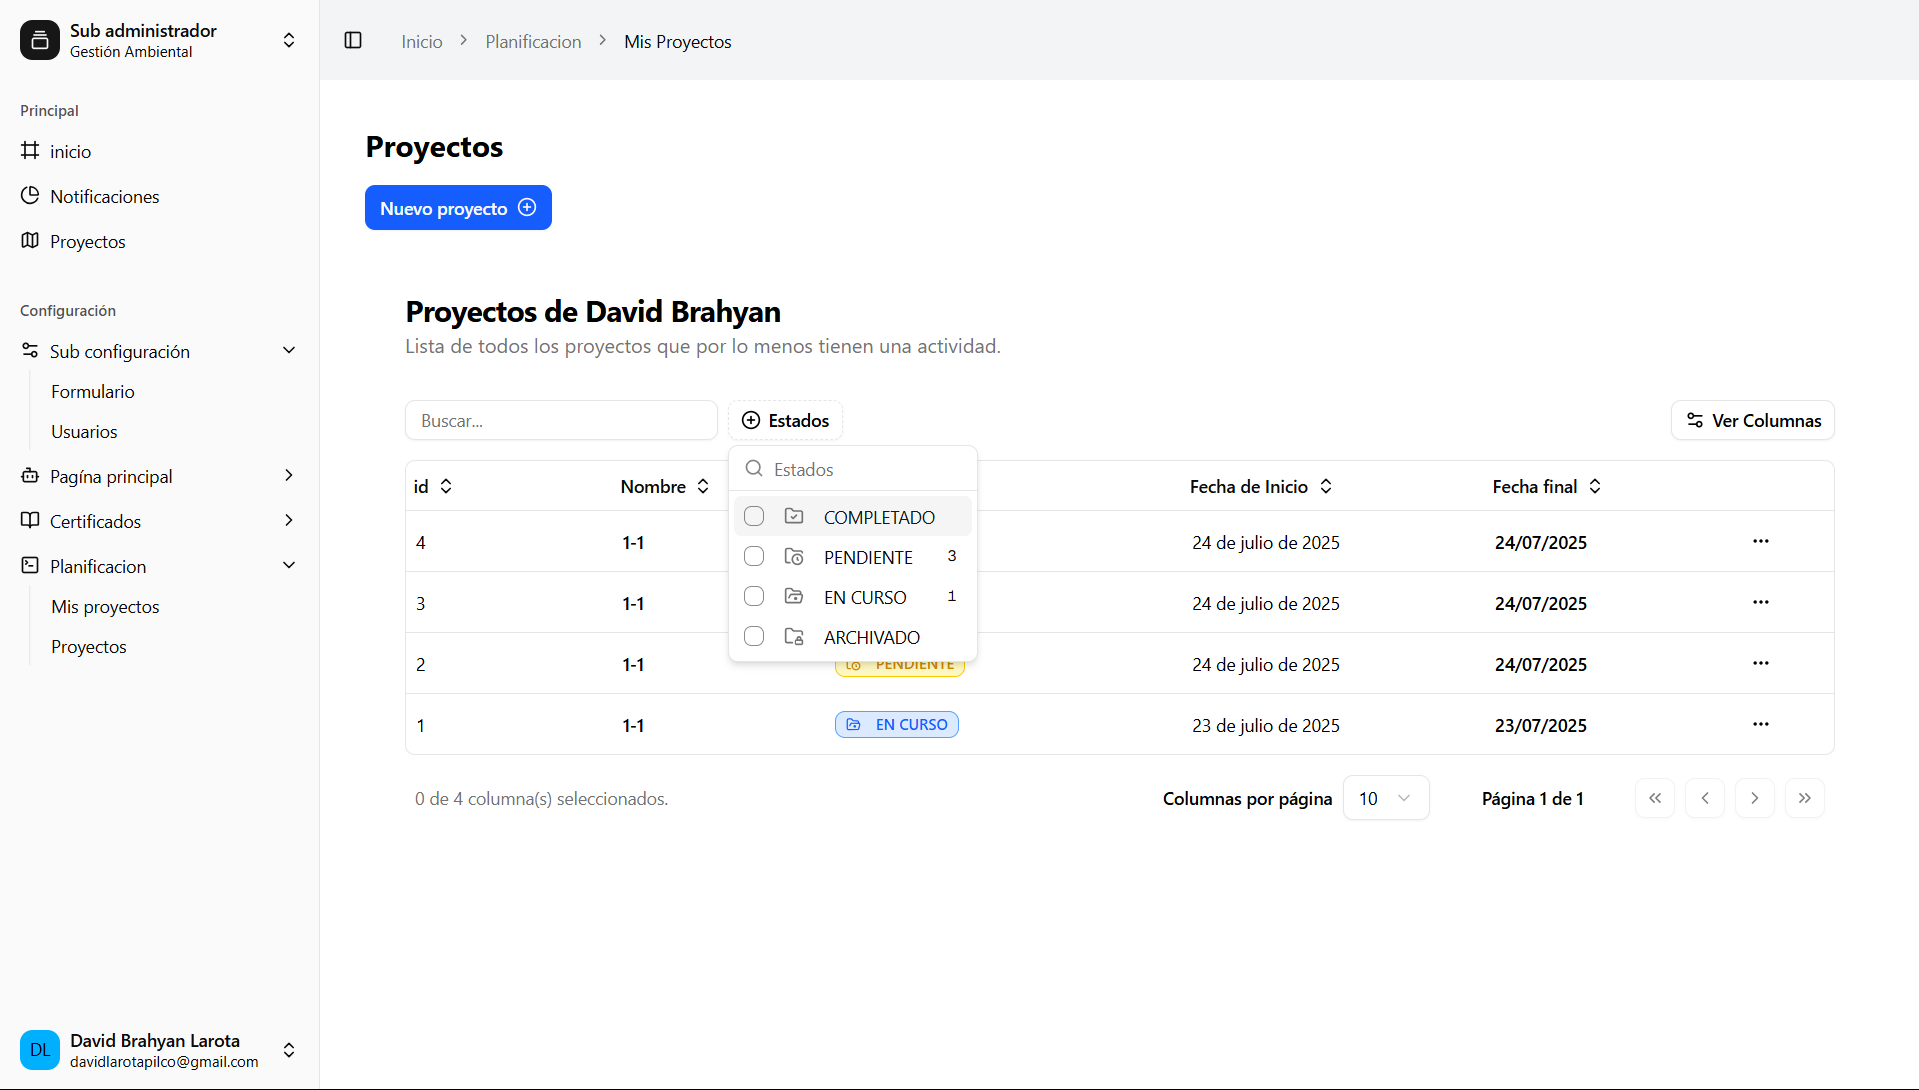
\includegraphics[width=0.8\textwidth]{assets/imagenes/proyectos_new.png}
    \label{fig:proyectos_page} 
\end{figure} 
\FloatBarrier
\begin{figure}[!htb] 
    \centering 
    \caption{Pagina para subir proyectos} 
    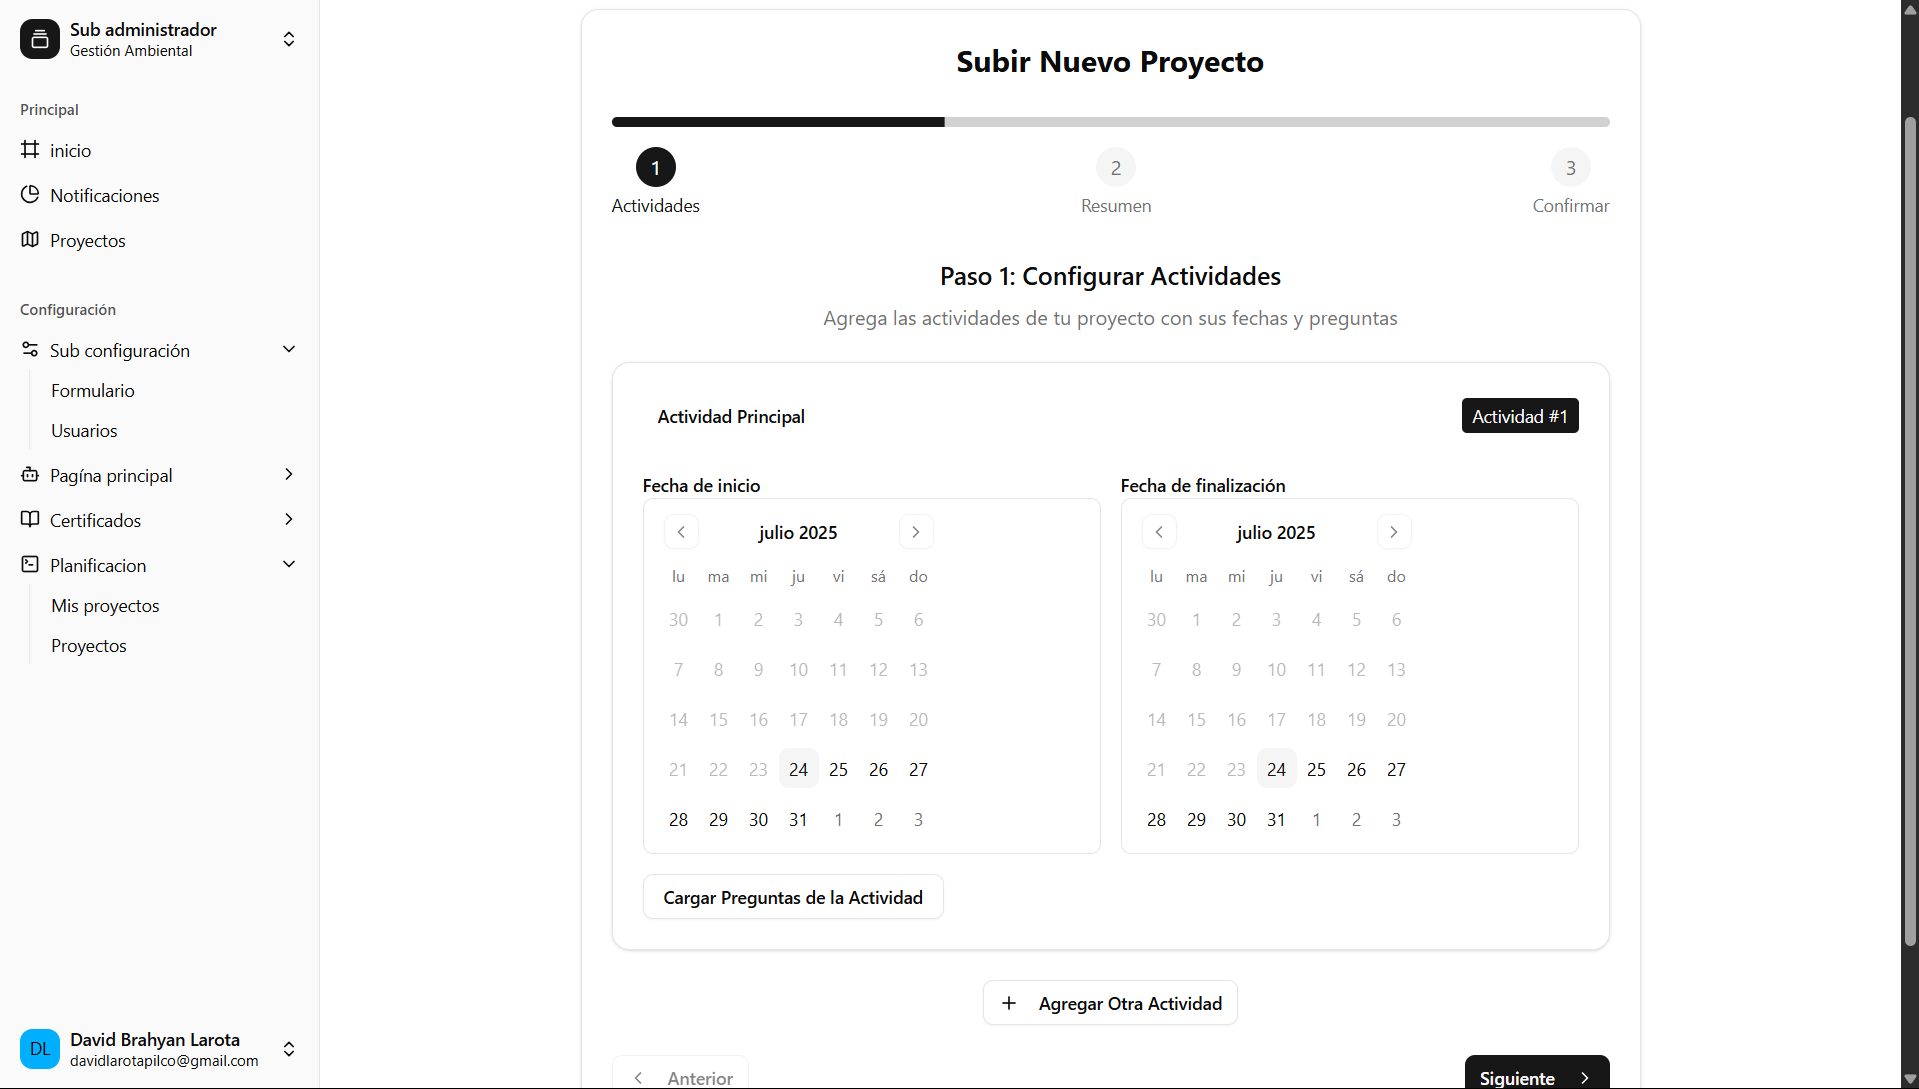
\includegraphics[width=0.8\textwidth]{assets/imagenes/subir_proyectos.png}
    \label{fig:subir_proyectos} 
\end{figure} 
\FloatBarrier
\begin{figure}[!htb] 
    \centering 
    \caption{Apartado de cuenta usuario} 
    
\includegraphics[width=0.8\textwidth]{assets/imagenes/cuenta.png}
    \label{fig:usuario} 
\end{figure} 
\FloatBarrier
\begin{figure}[!htb] 
    \centering 
    \caption{Soporte para modo oscuro} 
    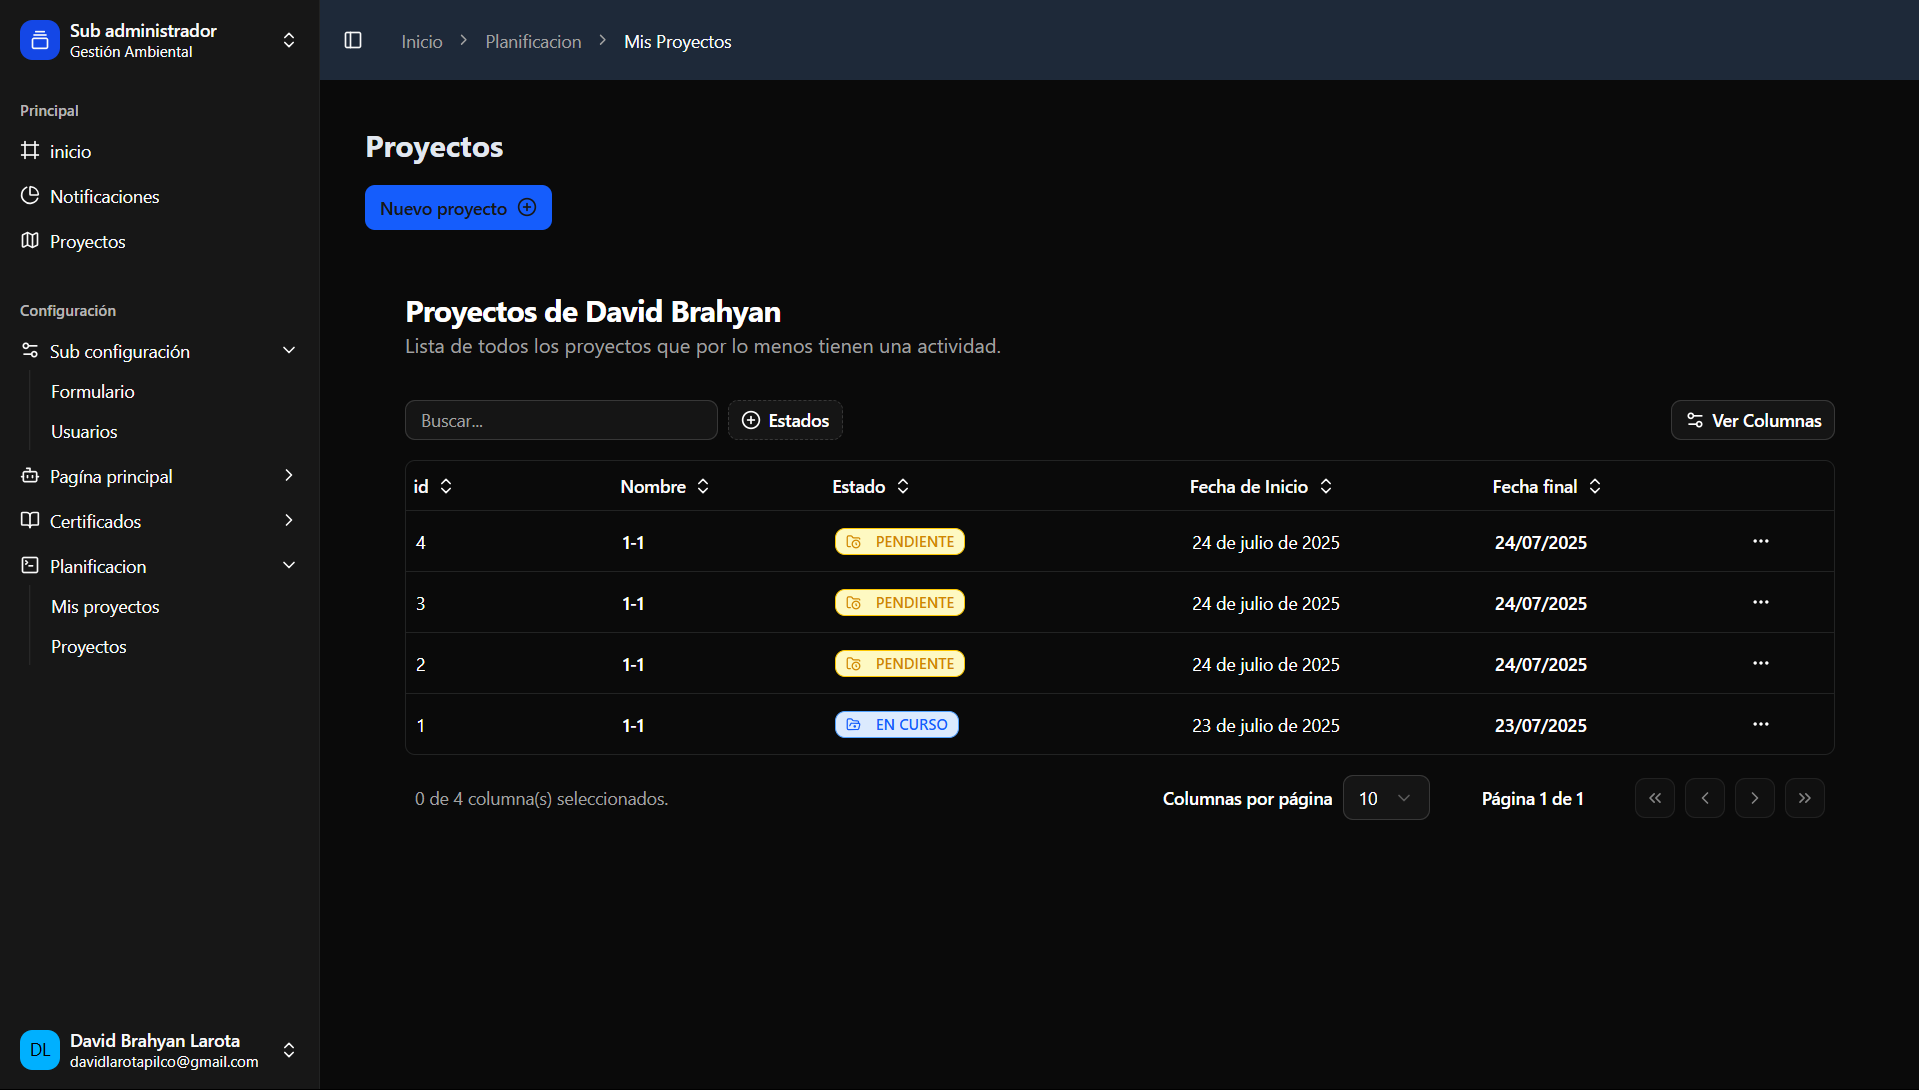
\includegraphics[width=0.8\textwidth]{assets/imagenes/modo_oscuro.png}
    \label{fig:modo_oscuro} 
\end{figure} 
\FloatBarrier
